\documentclass[aspectratio=169,9pt,t]{beamer}

\usepackage[T1]{fontenc}
\usepackage{lmodern}
\usepackage{amsmath,amssymb,mathtools}
\usepackage{graphicx}
\usepackage{tikz}
\usetikzlibrary{arrows.meta,positioning,calc,fit}

% A synchronized mechanism tutorial.  The right-hand method is a constructed
% fixed-step projected-gradient teaching control, not the retained native
% projected-GD endpoint used elsewhere in the project.

% ---------- palette ----------
\definecolor{Ink}{HTML}{172033}
\definecolor{Muted}{HTML}{5F6B7A}
\definecolor{Canvas}{HTML}{FAFAF7}
\definecolor{Graph}{HTML}{77736B}
\definecolor{BP}{HTML}{1769AA}
\definecolor{BPSoft}{HTML}{E8F2FA}
\definecolor{GD}{HTML}{087D77}
\definecolor{GDSoft}{HTML}{E5F5F2}
\definecolor{Gold}{HTML}{B85F00}
\definecolor{GoldSoft}{HTML}{FFF3D6}
\definecolor{Control}{HTML}{77736B}
\definecolor{ControlSoft}{HTML}{E7E5E0}

% ---------- Beamer setup ----------
\usetheme{default}
\usefonttheme{professionalfonts}
\setbeamertemplate{navigation symbols}{}
\setbeamercolor{normal text}{fg=Ink,bg=Canvas}
\setbeamercolor{frametitle}{fg=Ink,bg=Canvas}
\setbeamercolor{contrast}{fg=Ink,bg=GoldSoft}
\setbeamercolor{bpbox}{fg=Ink,bg=BPSoft}
\setbeamercolor{gdbox}{fg=Ink,bg=GDSoft}
\setbeamercolor{plainbox}{fg=Ink,bg=white}
\setbeamercolor{controlbox}{fg=Ink,bg=ControlSoft}
\setbeamersize{text margin left=5mm,text margin right=5mm}
\setbeamertemplate{frametitle}{%
  \vspace{.45mm}\insertframetitle\par
  \vspace{.15mm}{\color{Graph}\rule{\textwidth}{0.4pt}}\vspace{-2.3mm}}
\newcommand{\deckscope}{Exact sum-product BP vs constructed fixed-step projected-GD teaching control; synchronized beats do not imply equal arithmetic, memory, objectives, complexity, or iteration counts}
\setbeamertemplate{footline}{%
  \leavevmode\hbox{%
    \begin{beamercolorbox}[wd=.88\paperwidth,ht=2.5ex,dp=1.05ex,leftskip=5mm]{normal text}%
      \fontsize{5.25}{6.0}\selectfont\color{Muted}%
      \deckscope
    \end{beamercolorbox}%
    \begin{beamercolorbox}[wd=.12\paperwidth,ht=2.5ex,dp=1.05ex,rightskip=5mm plus 1fil]{normal text}%
      \fontsize{5.7}{6.3}\selectfont\color{Muted}%
      \insertframenumber/\inserttotalframenumber
    \end{beamercolorbox}}}

% ---------- fixed slide grammar ----------
\newcommand{\methodhead}[3]{%
  \begin{beamercolorbox}[rounded=true,sep=.6ex]{#1}
    \begin{columns}[T,onlytextwidth]
      \column{.39\textwidth}
        \fontsize{10}{11}\selectfont\bfseries\textcolor{#2}{#3}
      \column{.59\textwidth}
        \raggedleft\fontsize{6.2}{6.8}\selectfont
  \end{columns}
  \end{beamercolorbox}}

\newcommand{\bphead}[1]{%
  \begin{beamercolorbox}[rounded=true,sep=.58ex]{bpbox}
    \fontsize{10}{11}\selectfont\bfseries\textcolor{BP}{Belief propagation (BP)}\par
    \vspace{.1ex}\fontsize{6.2}{6.8}\selectfont\color{Ink}#1
  \end{beamercolorbox}}

\newcommand{\gdhead}[1]{%
  \begin{beamercolorbox}[rounded=true,sep=.58ex]{gdbox}
    \fontsize{10}{11}\selectfont\bfseries\textcolor{GD}{Projected GD}\par
    \vspace{.1ex}\fontsize{6.2}{6.8}\selectfont\color{Ink}#1
  \end{beamercolorbox}}

\newcommand{\statebp}[1]{%
  \vspace{.45mm}\begin{beamercolorbox}[rounded=true,sep=.42ex]{plainbox}
    \fontsize{6.2}{6.8}\selectfont\textcolor{BP}{\bfseries STATE ENTERING BEAT}\quad #1
  \end{beamercolorbox}}

\newcommand{\stategd}[1]{%
  \vspace{.45mm}\begin{beamercolorbox}[rounded=true,sep=.42ex]{plainbox}
    \fontsize{6.2}{6.8}\selectfont\textcolor{GD}{\bfseries STATE ENTERING BEAT}\quad #1
  \end{beamercolorbox}}

\newcommand{\smallcard}[2]{%
  \begin{beamercolorbox}[rounded=true,sep=.55ex]{plainbox}
    \fontsize{6.4}{7.1}\selectfont\textcolor{#1}{\bfseries #2}
  \end{beamercolorbox}}

\newcommand{\contrast}[1]{%
  \vfill
  \begin{beamercolorbox}[wd=\textwidth,rounded=true,sep=.65ex]{contrast}
    \centering\fontsize{7.2}{8.0}\selectfont
    \textcolor{Gold}{\bfseries WHAT DIFFERS HERE?}\quad #1
  \end{beamercolorbox}
  \vspace{0mm}}

\newcommand{\panelcolumns}[2]{%
  \begin{columns}[T,onlytextwidth]
    \column{.492\textwidth}#1
    \column{.492\textwidth}#2
  \end{columns}}

% ---------- diagram vocabulary ----------
\tikzset{
  bpbit/.style={circle,draw=BP,fill=white,line width=1.1pt,minimum size=7.8mm,inner sep=0pt,font=\fontsize{6.4}{7}\selectfont\bfseries},
  bpcheck/.style={rectangle,draw=BP,fill=BPSoft,line width=1.1pt,minimum width=7.8mm,minimum height=6.9mm,rounded corners=1.2pt,inner sep=0pt,font=\fontsize{7}{7.5}\selectfont\bfseries},
  gdbit/.style={circle,draw=GD,fill=white,line width=1.1pt,minimum size=7.8mm,inner sep=0pt,font=\fontsize{6.4}{7}\selectfont\bfseries},
  gdcheck/.style={rectangle,draw=GD,fill=GDSoft,line width=1.1pt,minimum width=7.8mm,minimum height=6.9mm,rounded corners=1.2pt,inner sep=0pt,font=\fontsize{7}{7.5}\selectfont\bfseries},
  baseedge/.style={draw=Graph!55,line width=1.0pt},
  bpactive/.style={draw=BP!28,line width=3.0pt},
  gdactive/.style={draw=GD!25,line width=3.0pt},
  qarrow/.style={draw=BP,line width=1.65pt,dashed,-{Stealth[length=2.0mm]},shorten <=3.5mm,shorten >=3.2mm},
  uarrow/.style={draw=BP,line width=1.65pt,dashed,-{Stealth[length=2.0mm]},shorten <=3.2mm,shorten >=3.5mm},
  dependency/.style={draw=GD,line width=1.55pt,dashed},
  bpchip/.style={fill=white,draw=BP,rounded corners=1.3pt,inner xsep=1.3pt,inner ysep=.8pt,font=\fontsize{5.8}{6.3}\selectfont,text=Ink},
  gdchip/.style={fill=white,draw=GD,rounded corners=1.3pt,inner xsep=1.3pt,inner ysep=.8pt,font=\fontsize{5.8}{6.3}\selectfont,text=Ink},
  tempchip/.style={fill=GoldSoft,draw=Gold,dashed,rounded corners=1.3pt,inner xsep=1.3pt,inner ysep=.8pt,font=\fontsize{5.8}{6.3}\selectfont,text=Gold},
  loopbp/.style={draw=BP,fill=BPSoft,line width=1.0pt,rounded corners=2pt,minimum height=10mm,text width=29mm,align=center,font=\fontsize{6.7}{7.3}\selectfont},
  loopgd/.style={draw=GD,fill=GDSoft,line width=1.0pt,rounded corners=2pt,minimum height=9mm,text width=28mm,align=center,font=\fontsize{6.7}{7.3}\selectfont},
  looptemp/.style={draw=Gold,fill=GoldSoft,dashed,line width=1.0pt,rounded corners=2pt,minimum height=9mm,text width=28mm,align=center,font=\fontsize{6.7}{7.3}\selectfont},
  bparrow/.style={draw=BP,line width=1.25pt,-{Stealth[length=2.2mm]}},
  gdarrow/.style={draw=GD,line width=1.25pt,-{Stealth[length=2.2mm]}},
  goldarrow/.style={draw=Gold,line width=1.15pt,-{Stealth[length=2.2mm]}}
}

\newcommand{\bpgraphbase}{%
  \node[bpcheck] (A) at (-1.55,1.45) {$A$};
  \node[bpcheck] (B) at ( 1.55,1.45) {$B$};
  \node[bpbit] (b1) at (-2.75,0) {bit 1};
  \node[bpbit] (b2) at ( 0.00,0) {bit 2};
  \node[bpbit] (b3) at ( 2.75,0) {bit 3};
  \draw[baseedge] (A)--(b1); \draw[baseedge] (A)--(b2);
  \draw[baseedge] (B)--(b2); \draw[baseedge] (B)--(b3);
}

\newcommand{\gdgraphbase}{%
  \node[gdcheck] (A) at (-1.55,1.45) {$A$};
  \node[gdcheck] (B) at ( 1.55,1.45) {$B$};
  \node[gdbit] (b1) at (-2.75,0) {bit 1};
  \node[gdbit] (b2) at ( 0.00,0) {bit 2};
  \node[gdbit] (b3) at ( 2.75,0) {bit 3};
  \draw[baseedge] (A)--(b1); \draw[baseedge] (A)--(b2);
  \draw[baseedge] (B)--(b2); \draw[baseedge] (B)--(b3);
}

\newcommand{\highlightbptwo}{\node[draw=Gold,circle,line width=1.3pt,minimum size=9.6mm,inner sep=0pt] at (b2.center) {};}
\newcommand{\highlightgdtwo}{\node[draw=Gold,circle,line width=1.3pt,minimum size=9.6mm,inner sep=0pt] at (b2.center) {};}

\begin{document}

% --------------------------------------------------------------------------
\begin{frame}{Beat 1 of 7: Two loops on one Tanner graph}
\panelcolumns{
  \bphead{retains fixed $L[3]$ + current $U[4]$}
  \vspace{.6mm}
  \centering
  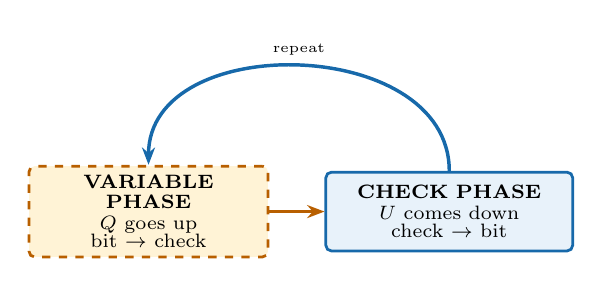
\begin{tikzpicture}[node distance=5mm]
    \node[looptemp] (var) {\textbf{VARIABLE PHASE}\\$Q$ goes up\\[-.2mm]bit $\to$ check};
    \node[loopbp,right=7mm of var] (chk) {\textbf{CHECK PHASE}\\$U$ comes down\\[-.2mm]check $\to$ bit};
    \draw[goldarrow] (var)--(chk);
    \draw[bparrow] (chk.north) to[out=90,in=90,looseness=1.15] node[above,font=\tiny]{repeat} (var.north);
  \end{tikzpicture}
  \vspace{-1.0mm}
  \[
    Q^{(t)}_{i\to c}=L_i+
      \sum_{d\in N(i)\setminus\{c\}}U^{(t-1)}_{d\to i}
  \]
  \smallcard{BP}{Each outgoing value retains a recipient address.}
}{
  \gdhead{retains fixed $\boldsymbol\ell[3]$ + current $\mathbf x[3]$}
  \vspace{.6mm}
  \centering
  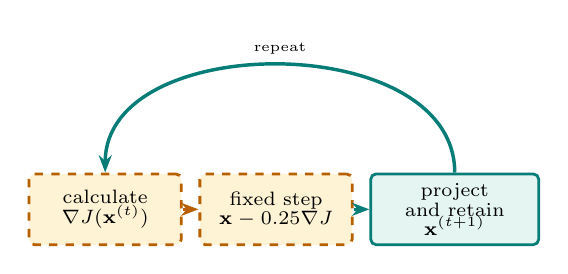
\begin{tikzpicture}[node distance=1.7mm]
    \node[looptemp,text width=17mm] (eval) {calculate\\$\nabla J(\mathbf x^{(t)})$};
    \node[looptemp,text width=17mm,right=2mm of eval] (step) {fixed step\\[-.2mm]$\mathbf x-0.25\nabla J$};
    \node[loopgd,text width=19mm,right=2mm of step] (proj) {project and retain\\[-.2mm]$\mathbf x^{(t+1)}$};
    \draw[goldarrow] (eval)--(step);
    \draw[gdarrow] (step)--(proj);
    \draw[gdarrow] (proj.north) to[out=90,in=90,looseness=1.05] node[above,font=\tiny]{repeat} (eval.north);
  \end{tikzpicture}
  \vspace{-1.25mm}
  \[
    \mathbf x^{(t+1)}=\Pi_{[-1,1]^3}
      \!\left(\mathbf x^{(t)}-0.25\nabla J(\mathbf x^{(t)})\right)
  \]
  \smallcard{GD}{$J(\mathbf x)=-\tfrac12\boldsymbol\ell^{\mathsf T}\mathbf x
    +2\!\left[(1-x_1x_2)^2+(1-x_2x_3)^2\right]$}
}
\contrast{Both methods use the graph, but BP advances edge-addressed messages while projected GD updates one scalar per bit.}
\end{frame}

% --------------------------------------------------------------------------
\begin{frame}{Beat 2 of 7: Store \texorpdfstring{$L_1,L_2,L_3$}{L1, L2, L3}; initialize all \texorpdfstring{$U^{(0)}_{c\to i}=0$}{U(c to i, 0)=0}}
\panelcolumns{
  \bphead{four directed edge values start at zero}
  \statebp{$\mathbf L=(-2.197,+0.405,+0.693)$; $\mathbf U^{(0)}=(0,0,0,0)$}
  \vspace{.4mm}\centering
  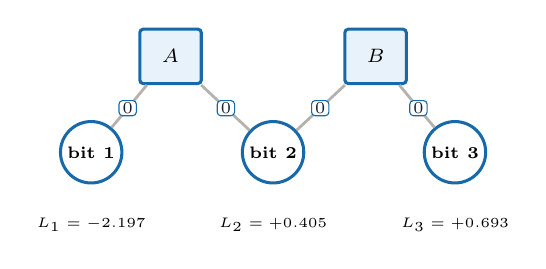
\begin{tikzpicture}[x=.84cm,y=.84cm]
    \bpgraphbase
    \node[bpchip] at ($(A)!.54!(b1)$) {$0$};
    \node[bpchip] at ($(A)!.54!(b2)$) {$0$};
    \node[bpchip] at ($(B)!.54!(b2)$) {$0$};
    \node[bpchip] at ($(B)!.54!(b3)$) {$0$};
    \node[below=3mm of b1,font=\tiny] {$L_1=-2.197$};
    \node[below=3mm of b2,font=\tiny] {$L_2=+0.405$};
    \node[below=3mm of b3,font=\tiny] {$L_3=+0.693$};
  \end{tikzpicture}
  \smallcard{BP}{\textbf{Stored before BP iteration 1:} $L[3]+U^{(0)}[4]=7$ values.}
}{
  \gdhead{one relaxed scalar is initialized per bit}
  \stategd{$\boldsymbol\ell=-\mathbf L$; $\mathbf x^{(0)}=\tanh(\boldsymbol\ell/2)$}
  \vspace{.4mm}\centering
  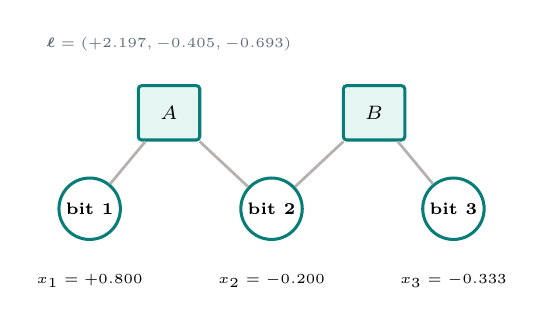
\begin{tikzpicture}[x=.84cm,y=.84cm]
    \gdgraphbase
    \node[below=3mm of b1,font=\tiny] {$x_1=+0.800$};
    \node[below=3mm of b2,font=\tiny] {$x_2=-0.200$};
    \node[below=3mm of b3,font=\tiny] {$x_3=-0.333$};
    \node[above=3mm of A,font=\tiny,text=Muted] {$\boldsymbol\ell=(+2.197,-0.405,-0.693)$};
  \end{tikzpicture}
  \smallcard{GD}{\textbf{Stored before the first GD update:} $\boldsymbol\ell[3]+\mathbf x^{(0)}[3]=6$ values.}
}
\contrast{The declared sign relation is $\boldsymbol\ell=-\mathbf L$. BP initializes directed edge state; projected GD initializes one scalar per bit.}
\end{frame}

% --------------------------------------------------------------------------
\begin{frame}{Beat 3 of 7: Variable-node stage forms \texorpdfstring{$Q^{(1)}_{i\to c}$}{Q(i to c, 1)} upward}
\panelcolumns{
  \bphead{forms four addressed $Q^{(1)}$ messages}
  \statebp{$\mathbf U^{(0)}=(0,0,0,0)$ remains frozen during this variable phase}
  \vspace{.6mm}\centering
  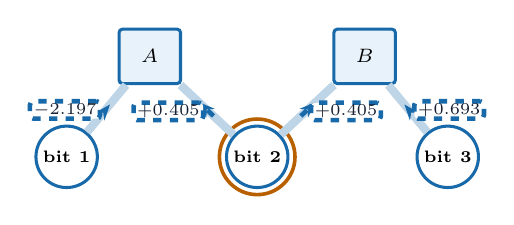
\begin{tikzpicture}[x=.88cm,y=.88cm]
    \bpgraphbase \highlightbptwo
    \draw[bpactive] (b1)--(A); \draw[bpactive] (b2)--(A);
    \draw[bpactive] (b2)--(B); \draw[bpactive] (b3)--(B);
    \draw[qarrow] (b1)--node[bpchip,pos=.47,left=.4mm] {$-2.197$}(A);
    \draw[qarrow] (b2)--node[bpchip,pos=.47,left=.4mm] {$+0.405$}(A);
    \draw[qarrow] (b2)--node[bpchip,pos=.47,right=.4mm] {$+0.405$}(B);
    \draw[qarrow] (b3)--node[bpchip,pos=.47,right=.4mm] {$+0.693$}(B);
  \end{tikzpicture}
  \vspace{.2mm}
  \[
    \mathbf Q^{(1)}=(-2.197,\ +0.405,\ +0.405,\ +0.693)
  \]
}{
  \gdhead{calculates two temporary check residuals}
  \stategd{$\mathbf x^{(0)}=(+0.800,-0.200,-0.333)$ remains frozen}
  \vspace{.6mm}\centering
  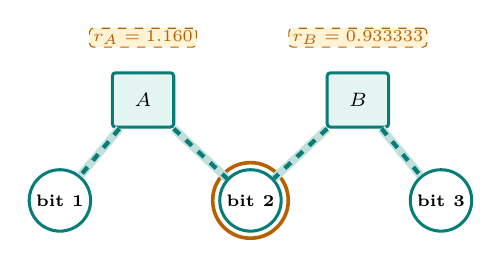
\begin{tikzpicture}[x=.88cm,y=.88cm]
    \gdgraphbase \highlightgdtwo
    \draw[gdactive] (A)--(b1); \draw[gdactive] (A)--(b2);
    \draw[gdactive] (B)--(b2); \draw[gdactive] (B)--(b3);
    \draw[dependency] (A)--(b1); \draw[dependency] (A)--(b2);
    \draw[dependency] (B)--(b2); \draw[dependency] (B)--(b3);
    \node[tempchip,above=3mm of A] {$r_A=1.160$};
    \node[tempchip,above=3mm of B] {$r_B=0.933333$};
  \end{tikzpicture}
  \vspace{.2mm}
  \[
    r_c=1-\prod_{j\in c}x_j,\qquad (r_A,r_B)=(1.160,0.933333)
  \]
}
\contrast{BP arrowheads show values travelling to named recipients. GD dashed lines show mathematical dependence, not travelling messages.}
\end{frame}

% --------------------------------------------------------------------------
\begin{frame}{Beat 4 of 7: Check-node stage forms \texorpdfstring{$U^{(1)}_{c\to i}$}{U(c to i, 1)} downward}
\panelcolumns{
  \bphead{new $U^{(1)}$ messages become directed state}
  \statebp{each degree-two check reads its pair of $Q^{(1)}$ messages}
  \vspace{.55mm}\centering
  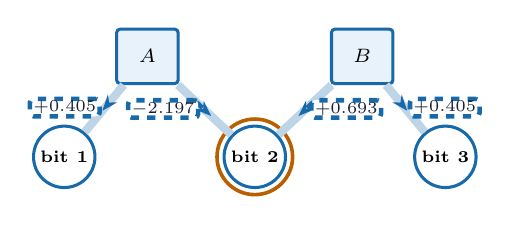
\begin{tikzpicture}[x=.88cm,y=.88cm]
    \bpgraphbase \highlightbptwo
    \draw[bpactive] (A)--(b1); \draw[bpactive] (A)--(b2);
    \draw[bpactive] (B)--(b2); \draw[bpactive] (B)--(b3);
    \draw[uarrow] (A)--node[bpchip,pos=.48,left=.4mm] {$+0.405$}(b1);
    \draw[uarrow] (A)--node[bpchip,pos=.48,left=.4mm] {$-2.197$}(b2);
    \draw[uarrow] (B)--node[bpchip,pos=.48,right=.4mm] {$+0.693$}(b2);
    \draw[uarrow] (B)--node[bpchip,pos=.48,right=.4mm] {$+0.405$}(b3);
  \end{tikzpicture}
  \vspace{.2mm}
  \[
    \mathbf U^{(1)}=(+0.405,-2.197,+0.693,+0.405)
  \]
}{
  \gdhead{four temporary terms contribute to the gradient}
  \stategd{all $g_{c,i}$ use the frozen $\mathbf x^{(0)}$ and residual $r_c$}
  \vspace{.25mm}\centering
  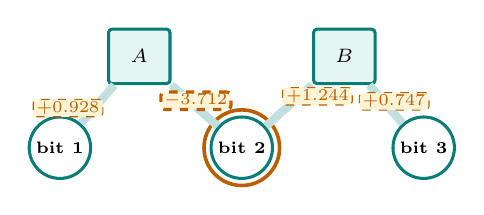
\begin{tikzpicture}[x=.84cm,y=.80cm]
    \gdgraphbase \highlightgdtwo
    \draw[gdactive] (A)--(b1); \draw[gdactive] (A)--(b2);
    \draw[gdactive] (B)--(b2); \draw[gdactive] (B)--(b3);
    \node[tempchip] at ($(A)!.58!(b1)+(-.38,.02)$) {$+0.928$};
    \node[tempchip,line width=1.15pt,fill=GoldSoft]
      at ($(A)!.52!(b2)+(.05,.05)$) {$-3.712$};
    \node[tempchip] at ($(B)!.52!(b2)+(.40,.12)$) {$+1.244$};
    \node[tempchip] at ($(B)!.52!(b3)+(.13,.04)$) {$+0.747$};
  \end{tikzpicture}
  \vspace{.2mm}
  \[
    g_{c,i}=-4r_c\!\prod_{\substack{j\in c\\j\ne i}}x_j
  \]
}
\contrast{BP retains four directed messages. In GD, $g_{A,1}$ contributes to $\partial J/\partial x_1$; $g_{A,2}$ and $g_{B,2}$ contribute to $\partial J/\partial x_2$; and $g_{B,3}$ contributes to $\partial J/\partial x_3$.}
\end{frame}

% --------------------------------------------------------------------------
\begin{frame}{Beat 4 continued: Compute \texorpdfstring{$g_{A,2}$}{g(A,2)}}
\panelcolumns{
  \bphead{the completed check-to-variable messages remain stored}
  \statebp{BP does not advance on this continuation slide}
  \vspace{.35mm}\centering
  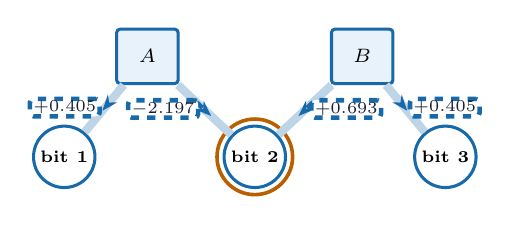
\begin{tikzpicture}[x=.88cm,y=.88cm]
    \bpgraphbase \highlightbptwo
    \draw[bpactive] (A)--(b1); \draw[bpactive] (A)--(b2);
    \draw[bpactive] (B)--(b2); \draw[bpactive] (B)--(b3);
    \draw[uarrow] (A)--node[bpchip,pos=.48,left=.4mm] {$+0.405$}(b1);
    \draw[uarrow] (A)--node[bpchip,pos=.48,left=.4mm] {$-2.197$}(b2);
    \draw[uarrow] (B)--node[bpchip,pos=.48,right=.4mm] {$+0.693$}(b2);
    \draw[uarrow] (B)--node[bpchip,pos=.48,right=.4mm] {$+0.405$}(b3);
  \end{tikzpicture}
  \vspace{.2mm}
  \[
    \mathbf U^{(1)}=(+0.405,-2.197,+0.693,+0.405)
  \]
}{
  \gdhead{specialize the general rule to one temporary term}
  \stategd{use the frozen $x_1=+0.800$, $x_2=-0.200$, and $r_A=1.160$}
  \vspace{-.15mm}\centering
  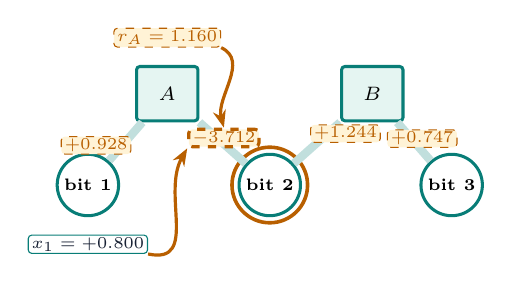
\begin{tikzpicture}[x=.84cm,y=.80cm]
    \gdgraphbase \highlightgdtwo
    \draw[gdactive] (A)--(b1); \draw[gdactive] (A)--(b2);
    \draw[gdactive] (B)--(b2); \draw[gdactive] (B)--(b3);
    \node[tempchip] at ($(A)!.58!(b1)+(-.38,.02)$) {$+0.928$};
    \node[tempchip,line width=1.15pt,fill=GoldSoft] (ga2)
      at ($(A)!.52!(b2)+(.05,.05)$) {$-3.712$};
    \node[tempchip] at ($(B)!.52!(b2)+(.40,.12)$) {$+1.244$};
    \node[tempchip] at ($(B)!.52!(b3)+(.13,.04)$) {$+0.747$};
    \node[tempchip,above=2.2mm of A] (ra) {$r_A=1.160$};
    \node[gdchip,below=2.2mm of b1] (xone) {$x_1=+0.800$};
    \draw[goldarrow] (ra.south east) to[out=-25,in=105] (ga2.north);
    \draw[goldarrow]
      (xone.south east) to[out=-12,in=-120,looseness=1.18] (ga2.south west);
  \end{tikzpicture}
  \vspace{0mm}
  \begin{beamercolorbox}[rounded=true,sep=.35ex]{gdbox}
    \centering
    \fontsize{5.9}{6.5}\selectfont
    $g_{c,i}=-4r_c\!\displaystyle\prod_{\substack{j\in c\\j\ne i}}x_j$
    $\;\Longrightarrow\;$ $c=A,\ i=2,\ A=\{1,2\}$\\[-.1mm]
    $r_A=1-x_1x_2=1-(0.800)(-0.200)=1.160$\\[-.1mm]
    $g_{A,2}=-4r_Ax_1=-4(1.160)(0.800)=\mathbf{-3.712}$
  \end{beamercolorbox}
}
\end{frame}

% --------------------------------------------------------------------------
\begin{frame}{Beat 5 of 7: Two \texorpdfstring{$Q$}{Q} messages versus \texorpdfstring{$\partial J/\partial x_2$}{dJ/dx2}}
\panelcolumns{
  \bphead{bit 2 prepares a different value for each check}
  \statebp{$L_2=+0.405$, $U^{(1)}_{A\to2}=-2.197$, $U^{(1)}_{B\to2}=+0.693$}
  \vspace{1.0mm}
  \begin{beamercolorbox}[rounded=true,sep=.8ex]{bpbox}
    \centering\fontsize{7.6}{8.5}\selectfont
    \textbf{Send to $A$: leave out $A$'s preceding contribution}
    \[
      Q^{(2)}_{2\to A}=L_2+U^{(1)}_{B\to2}
      =0.405+0.693=\mathbf{+1.099}
    \]
  \end{beamercolorbox}
  \vspace{1mm}
  \begin{beamercolorbox}[rounded=true,sep=.8ex]{bpbox}
    \centering\fontsize{7.6}{8.5}\selectfont
    \textbf{Send to $B$: leave out $B$'s preceding contribution}
    \[
      Q^{(2)}_{2\to B}=L_2+U^{(1)}_{A\to2}
      =0.405-2.197=\mathbf{-1.792}
    \]
  \end{beamercolorbox}
}{
  \gdhead{three terms form $\partial J/\partial x_2$}
  \stategd{$g_{A,2}=-3.712$, $g_{B,2}=+1.244$, $-\ell_2/2=+0.203$}
  \vspace{1.0mm}\centering
  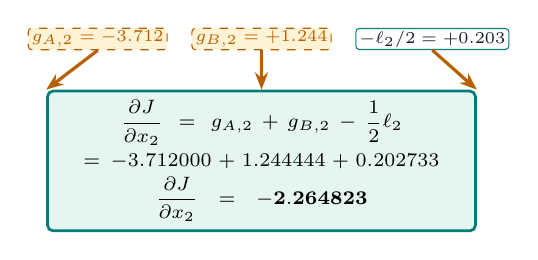
\begin{tikzpicture}[node distance=2mm]
    \node[tempchip] (ga) {$g_{A,2}=-3.712$};
    \node[tempchip,right=3mm of ga] (gb) {$g_{B,2}=+1.244$};
    \node[gdchip,right=3mm of gb] (ch) {$-\ell_2/2=+0.203$};
    \node[loopgd,text width=52mm,minimum height=13mm,below=5mm of gb] (sum)
      {$\displaystyle \frac{\partial J}{\partial x_2}
       =g_{A,2}+g_{B,2}-\frac12\ell_2$\\[.7mm]
       $\displaystyle =-3.712000+1.244444+0.202733$\\[.7mm]
       $\displaystyle \frac{\partial J}{\partial x_2}=\mathbf{-2.264823}$};
    \draw[goldarrow] (ga.south)--(sum.north west);
    \draw[goldarrow] (gb.south)--(sum.north);
    \draw[goldarrow] (ch.south)--(sum.north east);
  \end{tikzpicture}
  \vspace{1mm}
  \smallcard{GD}{$\partial J/\partial x_2$ is one number used to update $x_2$; GD does not form separate values addressed to $A$ and $B$.}
}
\contrast{For bit 2, BP forms $Q^{(2)}_{2\to A}$ and $Q^{(2)}_{2\to B}$ separately. GD sums $g_{A,2}$, $g_{B,2}$, and $-\ell_2/2$ to form $\partial J/\partial x_2$, which is used to update $x_2$.}
\end{frame}

% --------------------------------------------------------------------------
\begin{frame}{Beat 6 of 7: What the two checks read next}
\panelcolumns{
  \bphead{bit 2 presents two recipient-specific values}
  \statebp{the second variable phase has formed $\mathbf Q^{(2)}$}
  \vspace{.35mm}\centering
  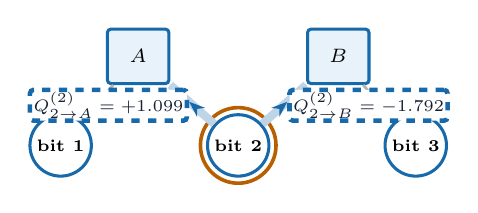
\begin{tikzpicture}[x=.82cm,y=.78cm]
    \bpgraphbase \highlightbptwo
    \draw[bpactive] (b2)--(A); \draw[bpactive] (b2)--(B);
    \draw[qarrow] (b2)--node[bpchip,pos=.48,left=.5mm] {$Q^{(2)}_{2\to A}=+1.099$}(A);
    \draw[qarrow] (b2)--node[bpchip,pos=.48,right=.5mm] {$Q^{(2)}_{2\to B}=-1.792$}(B);
  \end{tikzpicture}
  \vspace{.1mm}
  {\fontsize{7.2}{7.9}\selectfont\[
    \mathbf Q^{(2)}=(-2.197,+1.099,-1.792,+0.693)
  \]}
}{
  \gdhead{both checks read one updated bit-2 value}
  \stategd{$\nabla J(\mathbf x^{(0)})=(-0.171,-2.265,+1.093)$}
  \vspace{.35mm}\centering
  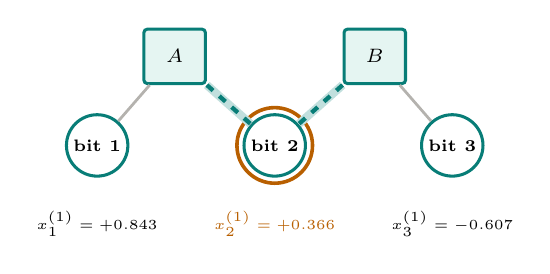
\begin{tikzpicture}[x=.82cm,y=.78cm]
    \gdgraphbase \highlightgdtwo
    \draw[gdactive] (A)--(b2); \draw[gdactive] (B)--(b2);
    \draw[dependency] (A)--(b2); \draw[dependency] (B)--(b2);
    \node[below=3mm of b1,font=\tiny] {$x_1^{(1)}=+0.843$};
    \node[below=3mm of b2,font=\tiny,text=Gold] {$x_2^{(1)}=+0.366$};
    \node[below=3mm of b3,font=\tiny] {$x_3^{(1)}=-0.607$};
  \end{tikzpicture}
  \vspace{.1mm}
  {\fontsize{7.0}{7.8}\selectfont
  \[
    \begin{aligned}
      \mathbf z^{(0)}&=\mathbf x^{(0)}-0.25\nabla J
        =(+0.843,+0.366,-0.607),\\
      \mathbf x^{(1)}&=\Pi_{[-1,1]^3}(\mathbf z^{(0)})=\mathbf z^{(0)}.
    \end{aligned}
  \]}
}
\contrast{This is the visible state boundary: BP has two addressed bit-2 values; projected GD retains one bit-2 scalar.}
\end{frame}

% --------------------------------------------------------------------------
\begin{frame}{Beat 7 of 7: What crosses the update boundary}
\panelcolumns{
  \bphead{boundary state: seven numerical values}
  \statebp{fixed $L[3]$ plus current directed $U^{(t)}[4]$}
  \vspace{1mm}
  \begin{beamercolorbox}[rounded=true,sep=.9ex]{bpbox}
    \centering
    \fontsize{11}{12}\selectfont\bfseries\textcolor{BP}{$L[3]+U^{(t)}[4]=7$}
    \par\vspace{1mm}
    \fontsize{7.1}{8}\selectfont
    Four separately addressed check-to-variable messages remain.\par
    $Q$ and $\boldsymbol\Lambda$ can be recalculated.
  \end{beamercolorbox}
  \vspace{1.2mm}
  \smallcard{BP}{Implementation note: $L[3]$ plus two four-position arrays allocates 11 positions; one degree-two conversion temporary gives peak 12.}
}{
  \gdhead{boundary state: six numerical values}
  \stategd{fixed $\boldsymbol\ell[3]$ plus current relaxed vector $\mathbf x^{(t)}[3]$}
  \vspace{1mm}
  \begin{beamercolorbox}[rounded=true,sep=.9ex]{gdbox}
    \centering
    \fontsize{11}{12}\selectfont\bfseries\textcolor{GD}{$\boldsymbol\ell[3]+\mathbf x^{(t)}[3]=6$}
    \par\vspace{1mm}
    \fontsize{7.1}{8}\selectfont
    Three current scalars remain, one for each bit.\par
    Residuals, $g_{c,i}$, $\nabla J$, and the trial point can be recalculated.
  \end{beamercolorbox}
  \vspace{1.2mm}
  \smallcard{GD}{Working-storage peak depends on implementation and is not included in the count of six.}
}
\contrast{The deck isolates a mechanism difference in representation, addressing, retention, and update. It does not establish which decoder performs better.}
\end{frame}

% ==========================================================================
% Controlled consequence: RQ2-GD-STATE-USE-001
\renewcommand{\deckscope}{RQ2-GD-STATE-USE-001: 200 paired held-out AWGN cases, 6 dB, 30 projected-GD updates; this bridge experiment does not rank native BP against native GD}

% --------------------------------------------------------------------------
\begin{frame}{From the state boundary to a causal test}
\begin{beamercolorbox}[rounded=true,sep=.65ex]{contrast}
  \centering\fontsize{7.4}{8.2}\selectfont
  \textcolor{Gold}{\bfseries RQ2 QUESTION}\quad
  If both projected-GD arms retain an offset $\delta_{c,i}$ for every Tanner-graph edge, does allowing the next update to \emph{use} those offsets change whether the hard decision equals the transmitted word?
\end{beamercolorbox}
\vspace{.8mm}

\begin{columns}[T,onlytextwidth]
  \column{.32\textwidth}
  \begin{beamercolorbox}[rounded=true,sep=.7ex]{bpbox}
    \fontsize{7}{7.8}\selectfont
    \textcolor{BP}{\bfseries WHAT THE TUTORIAL SHOWED}\par\vspace{.5mm}
    BP retains directed variable-to-check and check-to-variable messages.  The teaching projected-GD example retains one scalar per bit and recalculates terms from the parity checks.\par\vspace{.6mm}
    \textbf{That observation alone did not establish a performance consequence.}
  \end{beamercolorbox}

  \column{.65\textwidth}
  \begin{beamercolorbox}[rounded=true,sep=.65ex]{plainbox}
    \fontsize{6.7}{7.5}\selectfont
    \textcolor{Ink}{\bfseries HELD FIXED WITHIN EACH PAIR}\quad
    regular $(3,6)$ graph, transmitted word, received samples and channel LLRs, initialization, objective weights, preconditioner, backtracking procedure, 30-update budget, and hard-decision rule.
  \end{beamercolorbox}
  \vspace{.7mm}
  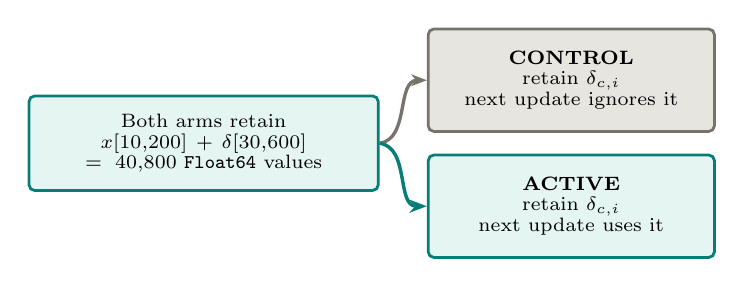
\begin{tikzpicture}[node distance=3mm]
    \node[loopgd,text width=42mm,minimum height=12mm] (state)
      {Both arms retain\\$x[10{,}200]+\delta[30{,}600]$\\$=40{,}800$ \texttt{Float64} values};
    \node[draw=Control,fill=ControlSoft,rounded corners=2pt,line width=1pt,
      text width=34mm,minimum height=13mm,align=center,font=\fontsize{6.7}{7.4}\selectfont,
      right=6mm of state,yshift=8mm] (control)
      {\textbf{CONTROL}\\retain $\delta_{c,i}$\\next update ignores it};
    \node[loopgd,text width=34mm,minimum height=13mm,
      right=6mm of state,yshift=-8mm] (active)
      {\textbf{ACTIVE}\\retain $\delta_{c,i}$\\next update uses it};
    \draw[-{Stealth[length=2mm]},draw=Control,line width=1.2pt] (state.east) to[out=8,in=180] (control.west);
    \draw[gdarrow] (state.east) to[out=-8,in=180] (active.west);
  \end{tikzpicture}
\end{columns}

\vfill
\begin{beamercolorbox}[rounded=true,sep=.55ex]{contrast}
  \centering\fontsize{7}{7.8}\selectfont
  This is a projected-GD bridge ablation study.  The offsets are not BP messages, and neither arm calls BP.
\end{beamercolorbox}
\end{frame}

% --------------------------------------------------------------------------
\begin{frame}{The controlled fork occurs at update 2}
\begin{beamercolorbox}[rounded=true,sep=.62ex]{plainbox}
  \centering\fontsize{7.4}{8.2}\selectfont
  \textbf{Entering update 2, all 200 pairs have exactly equal $\mathbf x^{(1)}$ and retained $\boldsymbol\delta^{(1)}$.}
\end{beamercolorbox}
\vspace{.8mm}

\begin{columns}[T,onlytextwidth]
  \column{.485\textwidth}
  \begin{beamercolorbox}[rounded=true,sep=.7ex]{controlbox}
    \fontsize{7.5}{8.3}\selectfont\textcolor{Control}{\bfseries CONTROL: RETAIN, DO NOT USE}\par
    \vspace{1mm}
    Each check reads
    \[
      \begin{aligned}
        s_{c,i}&=x_i,\\
        P_0(\mathbf x)&=\sum_c\left(1-\prod_{i\in c}x_i\right)^2 .
      \end{aligned}
    \]
    The scalar update is clipped to
    \[
      x_i^+\in[-1,1].
    \]
  \end{beamercolorbox}

  \column{.485\textwidth}
  \begin{beamercolorbox}[rounded=true,sep=.7ex]{gdbox}
    \fontsize{7.5}{8.3}\selectfont\textcolor{GD}{\bfseries ACTIVE: RETAIN AND USE}\par
    \vspace{1mm}
    Check $c$ reads its own shifted value
    \[
      \begin{aligned}
        s_{c,i}&=x_i+\delta_{c,i},\\
        P_\delta(\mathbf x)&=\sum_c\left(1-\prod_{i\in c}(x_i+\delta_{c,i})\right)^2 .
      \end{aligned}
    \]
    The bounds used by the projection keep every check reading in $[-1,1]$:
    \[
      x_i^+\in\left[\max_{c\ni i}(-1-\delta_{c,i}),\ 
      \min_{c\ni i}(1-\delta_{c,i})\right].
    \]
  \end{beamercolorbox}
\end{columns}

\vfill
\begin{beamercolorbox}[rounded=true,sep=.6ex]{contrast}
  \centering\fontsize{7.1}{7.9}\selectfont
  \textcolor{Gold}{\bfseries ONE REGISTERED TREATMENT, TWO LINKED EFFECTS:}\quad
  the active arm changes both the parity calculation and the bounds used by the projection.
\end{beamercolorbox}
\end{frame}

% --------------------------------------------------------------------------
\begin{frame}{The trajectories separate at the intended boundary}
\centering
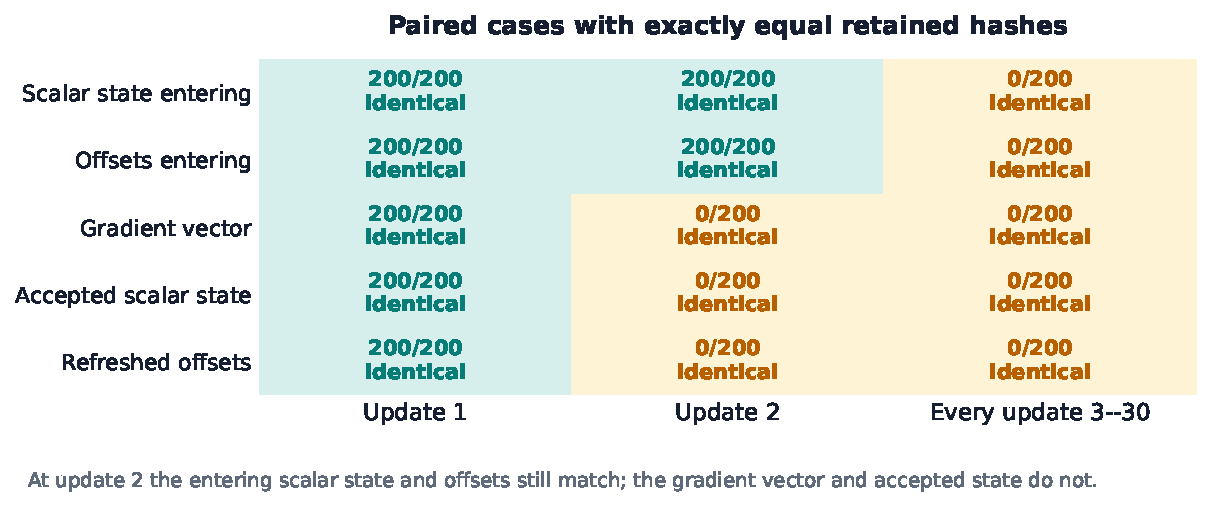
\includegraphics[width=.91\textwidth,height=.69\textheight,keepaspectratio]{figures/rq2_gd_state_use_001_divergence.pdf}

\vspace{-.5mm}
\begin{beamercolorbox}[wd=.96\textwidth,rounded=true,sep=.55ex]{gdbox}
  \fontsize{6.8}{7.5}\selectfont
  \textbf{Update 1:} all displayed quantities agree in 200/200 pairs.\quad
  \textbf{Update 2:} the entering state still agrees, but 0/200 gradient vectors and accepted scalar states agree.\quad
  The accepted step size remains equal in every pair, so it is not the first divergence.
\end{beamercolorbox}
\vspace{.4mm}
{\fontsize{5.8}{6.4}\selectfont\color{Muted}
Exact hash equality locates the first divergence; it does not measure the magnitude or desirability of that divergence.}
\end{frame}

% --------------------------------------------------------------------------
\begin{frame}{Using the retained offsets changes the result}
\centering
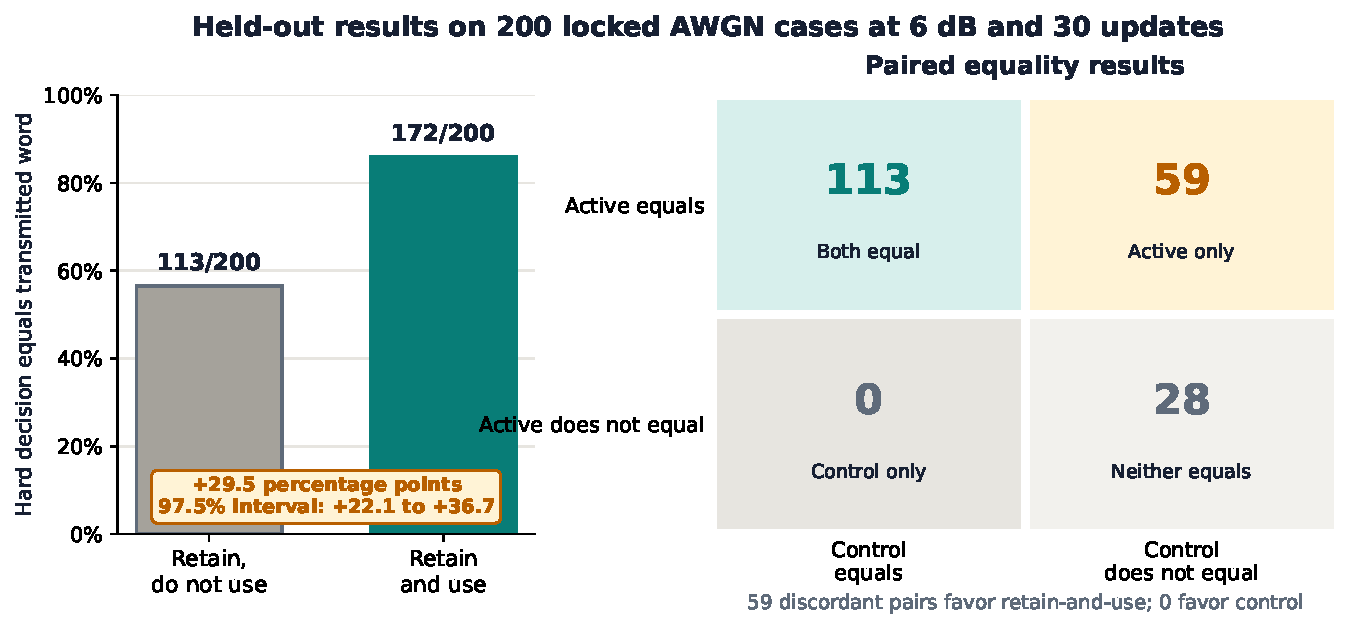
\includegraphics[width=.89\textwidth,height=.63\textheight,keepaspectratio]{figures/rq2_gd_state_use_001_recovery.pdf}

\vspace{-.8mm}
\begin{beamercolorbox}[wd=.97\textwidth,rounded=true,sep=.45ex]{plainbox}
  \fontsize{6.1}{6.8}\selectfont
  \textbf{Paired evidence:} exact McNemar $p=3.47\times10^{-18}$; Holm-adjusted $p=6.94\times10^{-18}$.  Whether the hard decision equals the transmitted word and whether it satisfies every parity check have the same paired table here; neither arm returns a wrong valid word.
\end{beamercolorbox}
\vspace{.15mm}
{\fontsize{5.3}{5.9}\selectfont\color{Muted}
Scope: one regular $(3,6)$ graph, 200 frozen held-out AWGN cases at physical $E_s/N_0=6$ dB, all-zero transmitted word, and 30 accepted updates.  This is not a BER-versus-SNR curve or a universal decoder ranking.}
\end{frame}

% --------------------------------------------------------------------------
\begin{frame}{What this contributes---and the next causal split}
\begin{beamercolorbox}[rounded=true,sep=.58ex]{gdbox}
  \centering\fontsize{7.1}{7.9}\selectfont
  \textbf{Both arms traverse the same Tanner graph and allocate the same persistent-state shape.}\quad
  Making the retained offsets usable changes the gradient vector, then the accepted scalar trajectory, then the final hard decision.
\end{beamercolorbox}
\vspace{.8mm}

\begin{columns}[T,onlytextwidth]
  \column{.50\textwidth}
  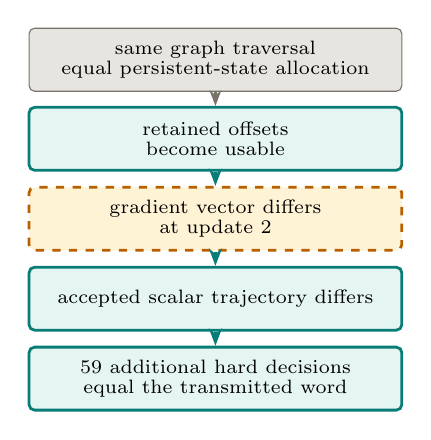
\begin{tikzpicture}[node distance=1.8mm]
    \node[draw=Control,fill=ControlSoft,rounded corners=2pt,text width=45mm,align=center,
      minimum height=8mm,font=\fontsize{6.7}{7.3}\selectfont] (graph)
      {same graph traversal\\equal persistent-state allocation};
    \node[loopgd,text width=45mm,minimum height=8mm,below=of graph] (use)
      {retained offsets\\become usable};
    \node[looptemp,text width=45mm,minimum height=8mm,below=of use] (derivative)
      {gradient vector differs\\at update 2};
    \node[loopgd,text width=45mm,minimum height=8mm,below=of derivative] (trajectory)
      {accepted scalar trajectory differs};
    \node[loopgd,text width=45mm,minimum height=8mm,below=of trajectory] (outcome)
      {59 additional hard decisions\\equal the transmitted word};
    \draw[-{Stealth[length=2mm]},draw=Control,line width=1pt] (graph)--(use);
    \draw[gdarrow] (use)--(derivative);
    \draw[gdarrow] (derivative)--(trajectory);
    \draw[gdarrow] (trajectory)--(outcome);
  \end{tikzpicture}

  \column{.47\textwidth}
  \begin{beamercolorbox}[rounded=true,sep=.58ex]{plainbox}
    \fontsize{7}{7.7}\selectfont\textcolor{Ink}{\bfseries NEXT: SPLIT THE BUNDLED TREATMENT}
  \end{beamercolorbox}
  \vspace{.5mm}
  \centering
  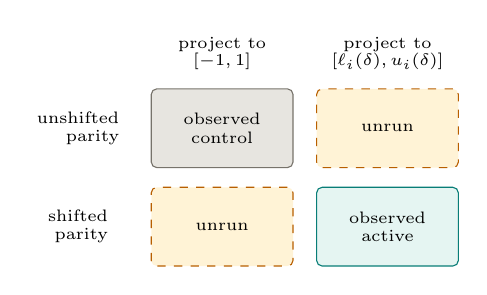
\begin{tikzpicture}[x=1cm,y=1cm]
    \node[font=\fontsize{5.8}{6.4}\selectfont,align=center] at (1.25,2.85) {project to\\$[-1,1]$};
    \node[font=\fontsize{5.8}{6.4}\selectfont,align=center] at (3.35,2.85) {project to\\$[\ell_i(\delta),u_i(\delta)]$};
    \node[font=\fontsize{5.8}{6.4}\selectfont,align=right] at (-.58,1.90) {unshifted\\parity};
    \node[font=\fontsize{5.8}{6.4}\selectfont,align=right] at (-.58,.65) {shifted\\parity};
    \node[draw=Control,fill=ControlSoft,rounded corners=2pt,minimum width=18mm,minimum height=10mm,
      align=center,font=\fontsize{6.2}{6.8}\selectfont] at (1.25,1.90) {observed\\control};
    \node[draw=Gold,fill=GoldSoft,dashed,rounded corners=2pt,minimum width=18mm,minimum height=10mm,
      align=center,font=\fontsize{6.2}{6.8}\selectfont] at (3.35,1.90) {unrun};
    \node[draw=Gold,fill=GoldSoft,dashed,rounded corners=2pt,minimum width=18mm,minimum height=10mm,
      align=center,font=\fontsize{6.2}{6.8}\selectfont] at (1.25,.65) {unrun};
    \node[draw=GD,fill=GDSoft,rounded corners=2pt,minimum width=18mm,minimum height=10mm,
      align=center,font=\fontsize{6.2}{6.8}\selectfont] at (3.35,.65) {observed\\active};
  \end{tikzpicture}
  \vspace{.2mm}
  \begin{minipage}{.95\linewidth}
    \centering\fontsize{6.2}{6.9}\selectfont\color{Muted}
    Only the diagonal cells have results.  The off-diagonal cells are the next proposed experiment.
  \end{minipage}
\end{columns}

\vfill
\begin{beamercolorbox}[rounded=true,sep=.52ex]{contrast}
  \centering\fontsize{6.7}{7.4}\selectfont
  \textbf{Not established:} that $\delta_{c,i}$ are BP messages, that retention alone caused the gain, that this reproduces BP, or that it uniquely explains the complete native BP--projected-GD gap.
\end{beamercolorbox}
\end{frame}

\end{document}
